% !TEX encoding = UTF-8 Unicode
\documentclass[a4paper,11pt,dvips]{article}

\usepackage[T1]{fontenc}
\usepackage[utf8]{inputenc}
\usepackage[british]{babel}
\usepackage[pdftex]{graphicx}
\usepackage{url}
\usepackage{natbib}
\usepackage{wrapfig}

\usepackage[margin=3cm]{geometry}

\begin{document}
\title{Forensics of Wearable Devices}
\author{Christoffer Hafsahl and Tommy Thorsen}
\maketitle


\begin{abstract}
In recent years, a new category of electronic gadgets has appeared, called \textit{wearables}. They are designed to be an integrated part of your daily life and track your movements throughout your day. What information can these devices reveal to the forensic analyst? We take a closer look at an Android Wear smartwatch and a popular activity tracker in order to find out.

This study provides examples of what data is available on these devices along with practical approaches to extracting this data.
\end{abstract}


\section{Introduction}

As the size of electronic components grow ever smaller, a new category of devices has emerged, called \textit{wearables}. Two types of wearables in particular, are beginning to see wide acceptance into mainstream use. These are the activity tracker and the smartwatch. In just a couple of years, they have gone from being novelty devices, ridiculed for "looking silly" and having ridiculously short battery life, to being genuinely desirable devices for a lot of people.

While the distinction between smartwatches and activity trackers can sometimes be a bit muddy -- some activity trackers are starting to adopt many smartwatch features and vice versa -- activity trackers tend to be less focused on user interface and more focused on the usefulness of their sensors. Smartwatches, on the other hand, tend to have some fitness-related features, but these are often fewer and more limited. Smartwatches do tend to have a larger screen, a more powerful GUI and usually a smartphone-like operating system.

What's common between the two types of devices, is that they are both worn on your wrist, and they are both meant to observe and measure the wearer throughout the day. They are also equipped with a variety of sensors for tracking activity, step counts, heart rate and other information about the wearer. Because of their close connection with the wearer, and focus on sensors and tracking, these new wearables could turn out to be a gold mine for the forensic analyst.

In this study, we want to take a closer look at how we can extract information from these wearable devices. We will investigate what data is available to us, and how this can possibly be used in an investigation. Wearables are seldom used completely independently -- they are usually synced with either a computer, a smartphone or to the cloud -- and we will also look at what data can be extracted from these other systems.

We have focused on two devices -- a smartwatch called \textit{LG Watch Urbane} and a activity tracker called \textit{Fitbit Charge HR}. We will dedicate sections to the findings for each of these devices after we've said a few words about the current state of forensic research for wearables.


\section{Background and Related Work}

Earlier this year, in August 2015, two independent studies were published on the subject of the forensics of smartwatches. The study \cite{baggili2015watch} sheds a lot of light on the forensics process of Android Wear and Samsung Gear smartwatches. \cite{rughanianalysis} is a short study outlining artifacts that may be of interest in the Android Wear platform.

Both of these studies, however, assume that the device can be \textit{rooted} in order to gain full access to the system. While this may be the case for some devices, most Android Wear devices can not be simply rooted. The chance that a device found in the wild is already rooted is also very slim. According to Google, less than 1\% of android smartphones are rooted \citep{Google:2014}. The authors of this study were not able to find a general method for rooting an android wear device without having to unlock the bootloader. The problem with unlocking the bootloader on any Android device (both watches and phones), completely wipes the memory of the device, eradicating any evidence we could hope to extract. In this study, we will explore what info can be extracted by the forensic analyst without rooting the device.

Smartwatches have a close relationship with smartphones. Android Wear devices demand to be paired with a smartphone as a part of the initial setup process, and acts much as an extension of the phone. The smartwatch is mainly used as a relatively passive device for displaying messages and other content pushed to it by the smartphone. We will therefore also spend some time looking at smartphone forensics in this study. \cite{hoog2011android} has literally written the textbook on Android forensics with his comprehensive and aptly named book "Android Forensics". Another, very useful, resource on android forensics is \cite{vidas2011toward}.

Although some research into digital forensics of activity trackers has been carried out, very little of it appears to be published. There has been at least one prior study on Fitbit, but this was specific towards the Fitbit Tracker, the first activity tracker from Fitbit. This model was based on the ANT+ communications platform and could only upload data by the use of a wireless base station connected to a computer. The computer kept clear-text logs of communication between the tracker and itself; and the data transmitted were unencrypted. Data uploaded to the Fitbit.com service was base-64-encoded but unencrypted, and was transmitted using HTTP (and not HTTPS). This allowed the researchers to reverse engineer the protocol between the base station and the tracker, and use this information to inject their own data into the device and to the website. \citep{rahman2013fit}

This is the only Fitbit device to use ANT+, so the research in that paper does not appear to be directly applicable to the tracker used in this article. Fitbit is also improving their software with new firmware releases every now and then; so their changes may also invalidate findings from the Rahman paper. Unfortunately there doesn’t seem to be a lot of published security-related research relevant for the newer Fitbit devices, so we’ve had to rely on work carried out by individual researchers and people involved with the tools used as part of this paper. There has also been some e-mail correspondence with French security researcher Axelle Aprville, who have done some investigation and a few presentations on Fitbit trackers. There are some studies such as \cite{lee2014validity} related to the accuracy of both Fitbit trackers and other brands, and while these can be relevant for investigators trying to determine how accurately the tracker categorizes various activities these do not appear to be relevant for us.


One of the most obviously useful types of data that may possibly be extracted from a wearable, is location data. \cite{maus2011forensic} contains a lot of useful information with regard to the extraction of geodata. As most wearables sync their data to the cloud, either via a smartphone or via a pc, the findings in \cite{chung2012digital} about cloud storage forensics are also very relevant to this study.

As wearable devices do contain a lot of personal and sensitive data, the producers of wearables have had to take steps to ensure that this data can not be easily stolen and abused. The security additions to recent fitbit devices have been well documented in \cite{cyr2014security}.


\section{LG Watch Urbane}

\begin{wrapfigure}{r}{0.4\textwidth}
\begin{center}
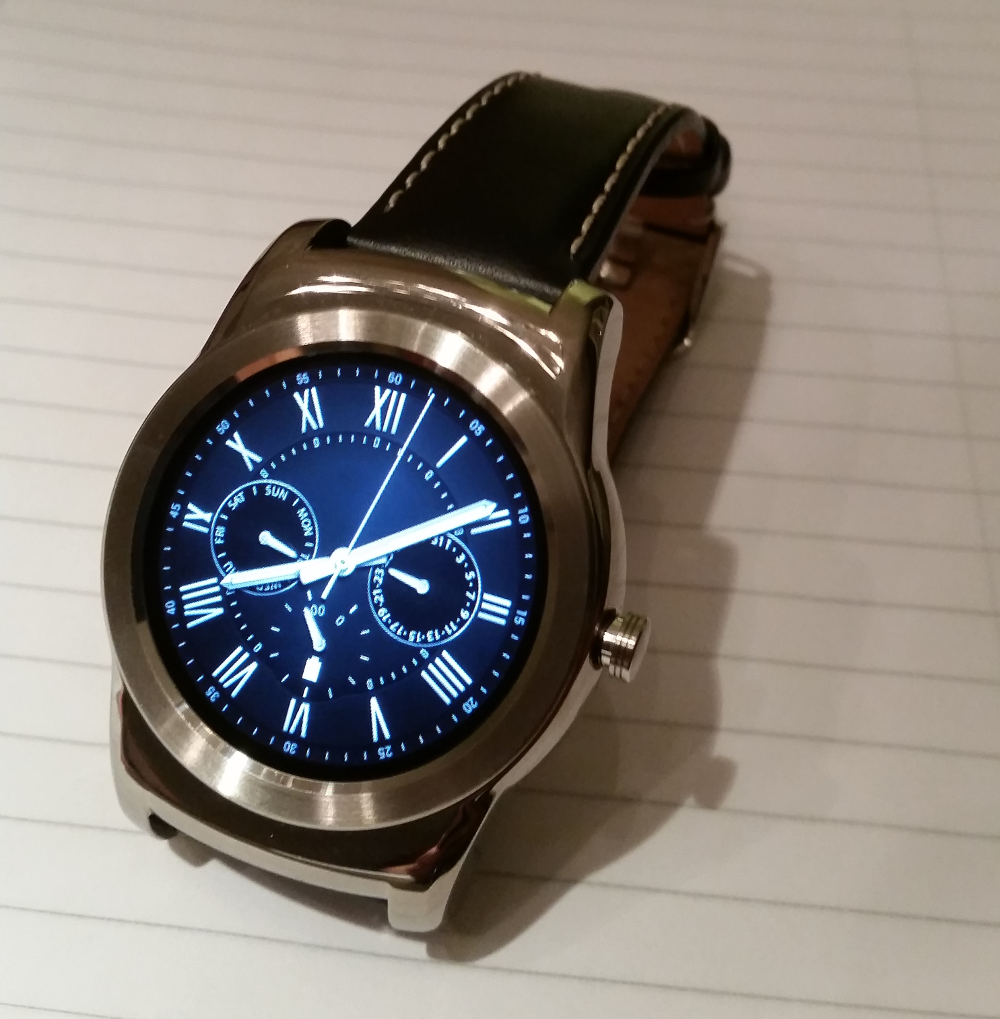
\includegraphics[natwidth=1000bp,natheight=1019bp,width=0.8\linewidth]{urbane}
\end{center}
\caption{The LG Watch Urbane.}
\label{fig:urbane}
\end{wrapfigure}

This smartwatch from LG is an Android Wear device. It is paired with a Samsung Galaxy S5. Neither of the devices are rooted. The watch comes with a 9-axis motion sensor and a sensor for measuring your heart rate. It comes with Google Fit preinstalled, and Google Fit uses the motion sensor to calculate daily step-counts for the wearer. There is unfortunately not any automatic heart rate monitoring -- if you want to know your heart rate, you have to manually initiate a measurement. This means that even if we are able to extract heart rate data from the watch, it will be of limited use.

Like all Android devices, it runs the Linux kernel with SELinux. Circumventing the security measures in an Android device is not trivial, and we are not going to attempt to hack the device in any way.


\subsection{Getting started with \texttt{adb}}

We mentioned earlier that we do not want to assume the device is rooted. This means we have to access the data we're interested in by other means than by making file system images. One good way to get fairly low-level access to Android devices, is by using the \textit{Android Debug Bridge}, or \texttt{adb}, which can be easiest acquired by installing the \textit{Android Studio} development environment.

In order to connect to any of our devices with \texttt{adb}, we need to turn on USB debugging inside the developer setting screen in the device. This unfortunately means we need to fiddle a bit with the device before we'll be able to extract any data. The procedure for enabling USB debugging is as follows:

\begin{enumerate}
\item Enter the "About device" screen which can be found inside the settings app.
\item Locate the "Build number" element and tap it seven times. You'll get a message saying that "Developer mode" has been activated.
\item Go back to the settings screen and enter the new "Developer options" screen.
\item Enable the "USB debugging" option.
\end{enumerate}

\noindent
Now you should be able to access your phone or watch via a USB cable. To test this, type \texttt{adb devices}. Your device should show up, something like this:

\scriptsize
\begin{verbatim}
$ adb devices
List of devices attached
db6c036d	device
\end{verbatim}
\normalsize


\subsection{Debug log acquisition}

A valuable, and often overlooked, source of information about an Android device, is the logging system. This is a collection of circular buffers in RAM that contain all sorts of information from various apps and from the operating system itself. They can be dumped to the terminal with the \texttt{adb logcat} command. A list of all the different debug buffers can be printed using the following command:

\scriptsize
\begin{verbatim}
$ adb logcat -g -b all
main: ring buffer is 256Kb (255Kb consumed), max entry is 5120b, max payload is 4076b
system: ring buffer is 256Kb (248Kb consumed), max entry is 5120b, max payload is 4076b
radio: ring buffer is 256Kb (19Kb consumed), max entry is 5120b, max payload is 4076b
events: ring buffer is 256Kb (254Kb consumed), max entry is 5120b, max payload is 4076b
crash: ring buffer is 256Kb (0b consumed), max entry is 5120b, max payload is 4076b
\end{verbatim}
\normalsize

In the \texttt{android} folder in the provided tools repository, there's a python script called \texttt{extract-logs} which can be used to automatically dump each of the available logs to a file along with the outputs of \texttt{adb shell dmesg} and \texttt{adb shell dumpsys}.

Since these logs are stored in circular buffers, the oldest log entries are constantly being overwritten by new information. It's not possible to say exactly how many hours worth of logs there are, because this depends on how verbose the software running on the device is, but typically around 5--8 hours worth of logs can be expected on an Android Wear device. There are usually fewer hours worth of logs available in an Android phone, because there is typically more software running, and more debug statements printed to the logs.

This makes the debug logs highly volatile information that should be acquired as soon as possible after getting hold of a live device. While it may be normal procedure to put the device straight into a faraday bag to avoid remove wiping of the device, this can actually be detrimental to the analysts ability to retrieve anything useful from the logging system. Not only are old log statements constantly being overwritten the entire time the phone is in the bag, but depriving the phone of network connection is likely to increase the flow of error messages printed to the logs. This will make old log statements be overwritten at a much higher rate than normal.

A good compromise might be to first put the device into a faraday bag, and then immediately plug the usb cable in and start the procedure for extracting the logs while the device is in the bag.


\subsection{The \texttt{WearableConn} log tag}

The first thing you may want to look for in the log, is the \texttt{WearableConn} tag. These debug lines can be found both on the watch and on the phone, and they can tell you when the two devices got separated or brought together again. When the watch and phone lose connection for any reason, for instance because they move out of range of each other, a line like the following will be printed to the main log:

\scriptsize
\begin{verbatim}
11-11 17:01:03.705 I/WearableConn(  774): Connection closed, waiting.
\end{verbatim}
\normalsize

\noindent
When the two devices are brought back together, the following line can be found in the log:

\scriptsize
\begin{verbatim}
11-11 17:06:14.011 I/WearableConn(  774): Connected, running sync loop
\end{verbatim}
\normalsize

\noindent
This can potentially be useful for determining what exact time an event happened. Let's imagine a hypothetical scenario.

\begin{quote}
\textit{At 18:00 the police receive a report about a missing person. A young girl left the house of a friend at 16:00, but never made it home. The exact time of disappearance is unknown. Her handbag, containing her smartphone, is found along the road and handed to the police. Since she is known to be wearing a smartwatch, we extract the logs from the phone and look for the WearableConn messages. We find the above line in the log, saying that the phone lost sight of the watch at 17:01.}

\textit{We now have a really exact time of disappearance, which should help the police a lot if they want to look through surveillance camera footage or calculate how far away a kidnapper might be.}
\end{quote}


\subsection{The \texttt{DisplayManagerService} log tag}

The \texttt{DisplayManagerService} log statements can sometimes be useful. Specifically, the following line can tell us something important:

\scriptsize
\begin{verbatim}
11-11 19:29:00.971 I/DisplayManagerService(  573): Display device changed state: "Built-in Screen", OFF
\end{verbatim}
\normalsize

\noindent
This line tells us that the screen has turned off. This can mean one of two things. If the "always-on screen" setting is true, it means that the watch has been lying still for 30 minutes, and the system has turned the screen off to save battery. The above log line then means that the watch was put down at around 18:59. If the "always-on screen" setting is false, then the screen will turn off after 5 seconds without receiving any touch events. In this case, the log will contain a lot of these \texttt{"Built-in Screen", OFF} lines. We can find the time the watch was put down by subtracting 5 seconds from the last of these events to appear in the log. Either way, we have a good way to find out how long a smartwatch has been lying still. Let's go back to our hypothetical kidnapping case:

\begin{quote}
\textit{Fast forward two hours. The time is now 20:00. We have acquired a description of the car the suspected kidnapper is driving. A car that matches this description is found abandoned near the edge of a forest. A police dog finds a smartwatch with a ripped wristband lying in the grass. We connect the watch to the pc, noticing that the "always-on screen" setting is on as we enable adb in the settings. The system log file shows us the above line, meaning that they must have passed through here at 18:59.}

\textit{We now know the kidnapper has a one hour head start on us, but he's on foot.}
\end{quote}


\subsection{Log file statistics}

Finally, we can take a step back and look at the log files in a different way. A device in active use generates more debug output than a device that's idling. By counting how many debug lines are printed during different periods of time, we can get some rough statistics on the activities on the user. Figure~\ref{fig:eventlog} shows a histogram created from the event log of the author's smartwatch.

\begin{figure}
\noindent
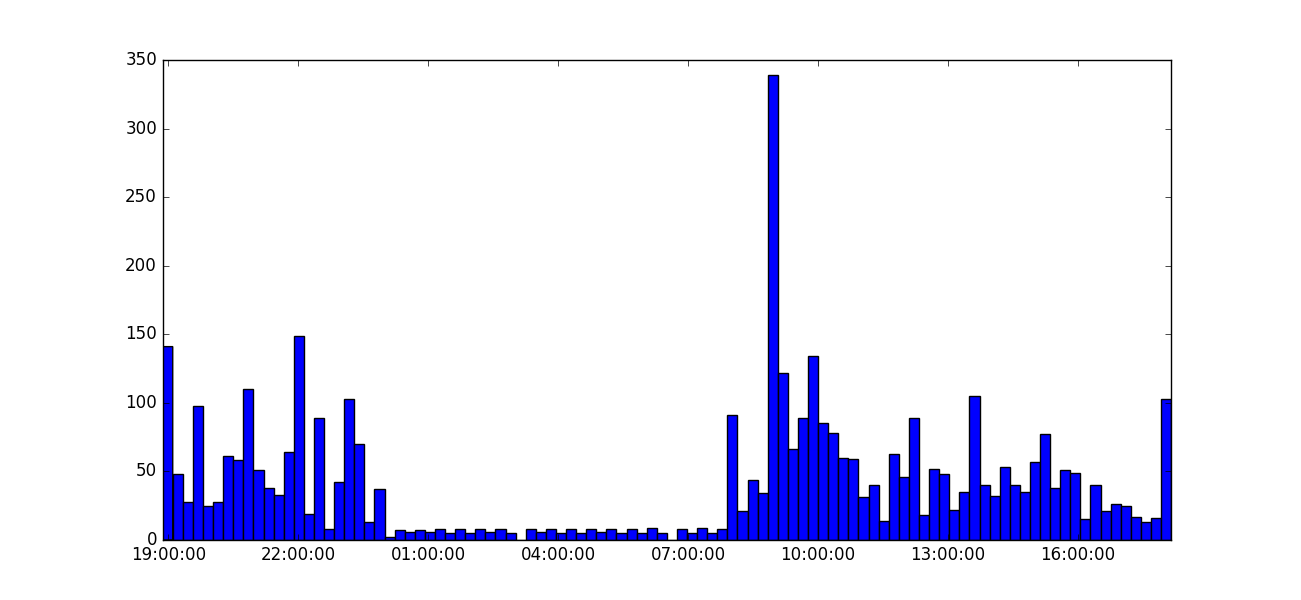
\includegraphics[natwidth=1301bp,natheight=600bp,width=\linewidth]{eventlog}
\caption{A histogram of events from an LG watch in normal use.}
\label{fig:eventlog}
\end{figure}

\noindent
The diagram shows quite clearly the time period when the author is sleeping. It also shows that the author does not sleep with the watch on his wrist. If that was the case, we would probably see more spurious activity from the watch at night, as the wearer moves.


\subsection{Extracting the filesystem}

We made an attempt at extracting the file system of the LG watch without root access, but we did not have much success. Using \texttt{adb pull}, it is possible to fetch all the files we have read access to. The authors were not able to recover much useful information from these files, however.

Likewise, using the \texttt{adb backup} command to extract files from the user partition of an non-rooted Android device turned out not to work on Android Wear. It appears the backup system has been disabled on most, if not all, Android Wear watches. We have still included a tool called \texttt{extract-files-by-adb-backup} because of its usefulness in extracting files from non-rooted phones.


\subsection{Extracting data from the Google Fit API}

We were originally thinking that we would be able to extract fitness data from database files on the filesystem, but since we did not have root access on the watch, and it was not possible to use \texttt{adb backup} to extract files from the user data partition, we had to think outside of the box. Why not use the mechanism Google intended for us to use, namely the Google Fit API?

We ended up writing an app that can be installed to either the phone or the watch. The app extracts data from the Google Fit API and dumps it to the logging system, where it can be picked up by a computer program and piped to a file. The app seems to be able to get more detailed data from the phone than from the watch, but it does not require communication between the devices. We are able to extract the data without any manual steps for the watch, and it works in airplane mode, meaning that it would work even if the watch was inside a faraday bag. We were not able to extract anything from the phone without internet access, as some manual authentication steps are required.

The data we are able to extract includes, but is not limited to: activity measurements, step counts, locations and heart rates. Wearables with more sensors would let us extract more types of data. As an example, figure~\ref{fig:stepcount} shows a diagram of step counts extracted from the author's smartwatch. We can see that most of the steps happen in the morning and in the afternoon. This pattern is consistent with the author walking to and from work every day. The smaller spikes, indicating shorter walks throughout the day, are likely to be coffee-related.

\begin{figure}
\noindent
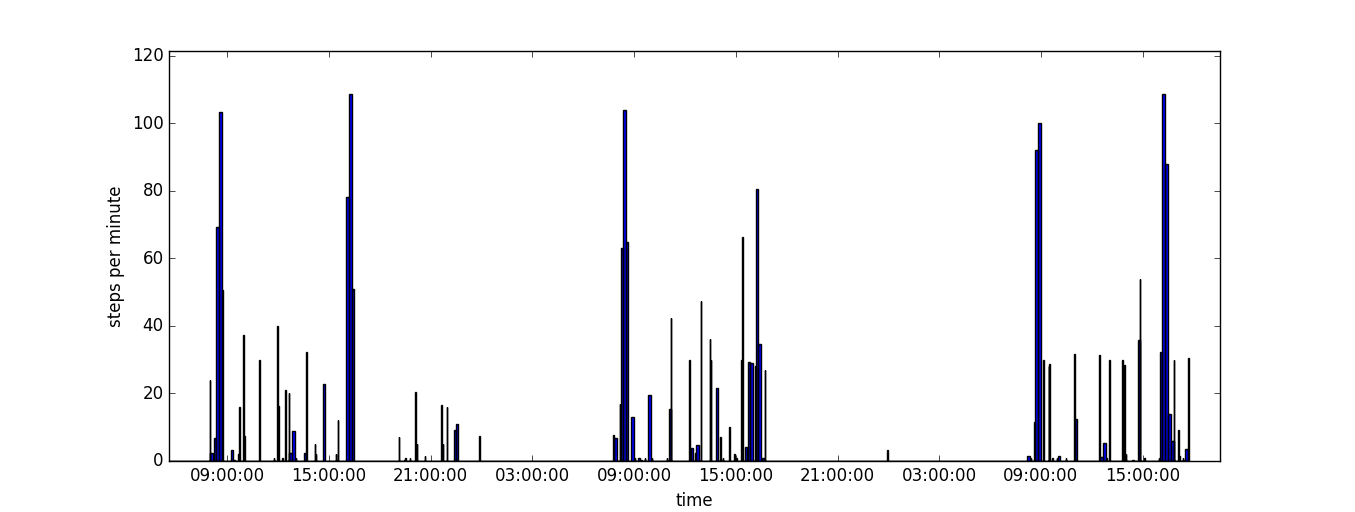
\includegraphics[natwidth=1355bp,natheight=512bp,width=\linewidth]{stepcount}
\caption{Histogram showing step counts per minute over three days.}
\label{fig:stepcount}
\end{figure}

The extracted xml file also contains location data. This data can be converted into a \textit{kml} file by the included tool \texttt{create-kml-from-fitness-data}. The resulting kml file can be opened in Google Maps, Google Earth or any other map software that supports this geodata file format. (See figure~\ref{fig:geodata}). This gives us an interactive timeline of the location of the wearable at regular intervals.

\begin{figure}
\noindent
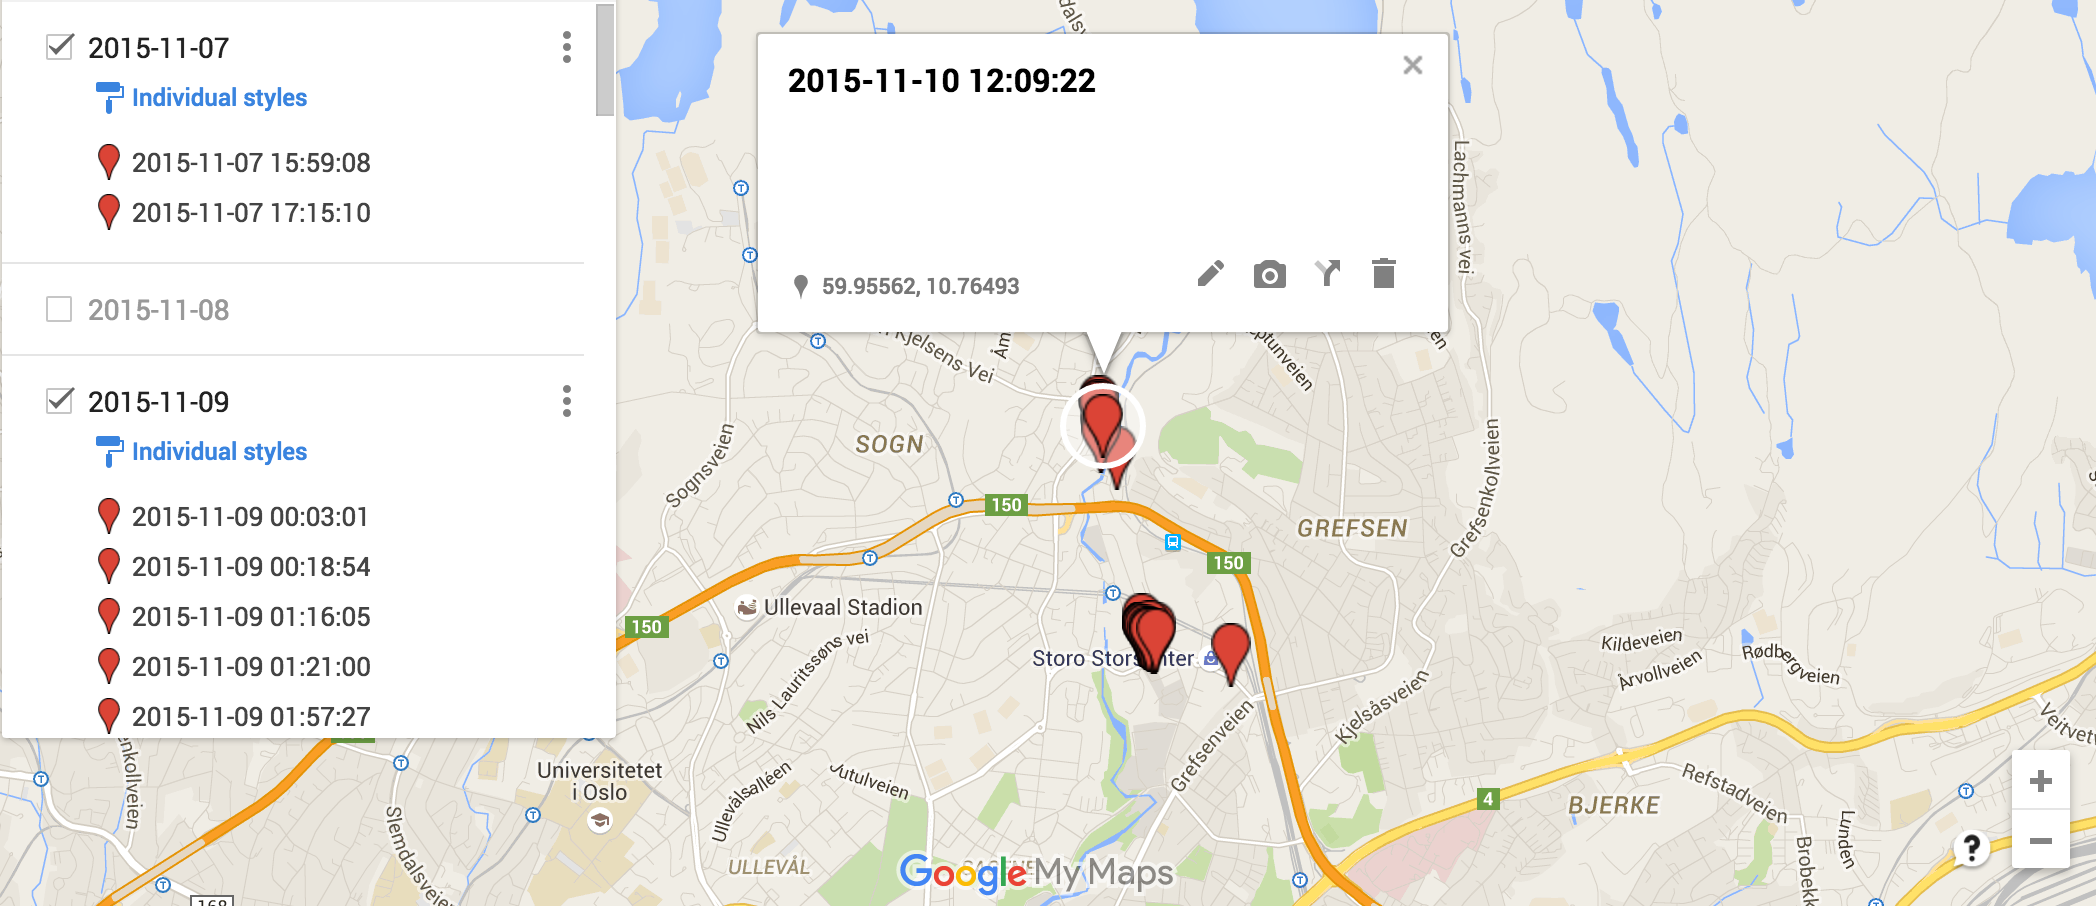
\includegraphics[natwidth=2096bp,natheight=906bp,width=\linewidth]{geodata}
\caption{The kml file containing the author's movements over the past 5 days, shown in Google Maps.}
\label{fig:geodata}
\end{figure}


\section{Fitbit Charge HR}

Data from activity trackers have already been part of at least one criminal case \citep{Snyder:2015} and one injury lawsuit \citep{Olson:2014}. As they become more mainstream we can expect to see more of these devices related to criminal and other investigations. If so, the data captured by the device can be important in terms of supporting other evidence or claims from victims or suspects, and also to help establish the timeline of a crime.

In order for us to better relate to information uncovered as part of this work, let's imagine two scenarios. The first one involves a murder victim; little is known about the person or events surrounding the death, but the body was found with an activity tracker attached and a paired smartphone. Can the tracker contain any useful information, and is it possible to extract the data from it or the smartphone? In another scenario we have a committed crime, and a person with a motive. S/he claims to be innocent, and the investigators discovers an activity tracker related to the person. Does this hold any useful data supporting or contradicting the alibi, and if so how trustworthy are the data?

To examine this, we decided to obtain a activity tracker and use it regularly for a period to generate data. The device chosen is the Charge HR from the company Fitbit; which according to the manual has a 3-axis accelerometer used to measure motion. This data is then used to count the number of steps taken, distance traveled, calories burned, as well as the wearers' sleep quality. In addition it also has an altimeter which is used to measure the number of floors climbed, and a heart rate sensor measuring the pulse. It captures data on a per-minute basis stored on the device for the past seven days, also keeping an average for each day for the past 30 days.

Although there are many similar devices on the market at present, the reasons for choosing this device were non-scientific and fairly basic:

\begin{description}
\item[Availability] several competing stores had multiple models from Fitbit in stock; most of them relatively inexpensive (<800,- NOK).
\item[Popularity] According to the sales representatives asked it was a fairly popular brand; the author had also heard about Fitbit prior to starting this paper, the company also claims to have sold more than 30 million devices \citep{Fitbit:2015}.
\item[Proprietary] It wasn't based on Android (as the LG Watch Urbane covers this), but uses proprietary software specific to this company.
\end{description}

\subsection{Fitbit ecosystem}
Although the activity tracker is capable of displaying the current number of steps, distance walked, pulse rate and floors climbed, it isn't possible to do much else on the device itself. Fitbit offers a free service on the website Fitbit.com, where users can access a “dashboard” (figure~\ref{fig:dash}) with visual representations of the captured data along with reports, interaction social networks such as Google+ and Facebook as well as various plans and goals. They also offer a paid “premium” service giving access to additional reports and functionality.

\begin{figure}
\begin{center}
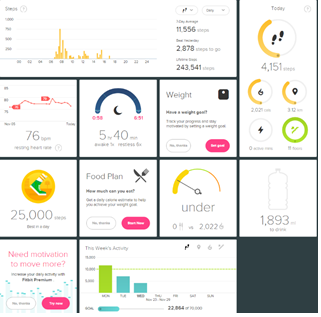
\includegraphics[natwidth=321bp,natheight=317bp,width=0.6\linewidth]{dash}
\end{center}
\caption{Fitbit.com dashboard with tiles representing various measurements, services and offers}
\label{fig:dash}
\end{figure}

To upload data to this service, the Fitbit device needs to be paired with a computer and/or a smartphone. Communication between the devices uses the Bluetooth Low Energy (BTLE) protocol, and once paired the user only has to be within range of the receiver. Although uploads can be initiated manually, no interaction is normally required. On smartphones Fitbit offers this upload functionality as part of an app which contains a similar dashboard to the one found on Fitbit.com, although with less features.

\subsection{Accessing the data}
There are multiple approaches one can take in order to access the captured data, all depending on how much effort, time and resources is available. But from the approaches identified, we decided on the following three:

\begin{itemize}
\item Extracting data from the device itself
\item Extracting data from the Fitbit API
\item Extracting the data from a paired smartphone
\end{itemize}

Fitbit doesn't support exports of the minute-by-minute data, also known as intraday data from the device itself, the mobile app or from the dashboard. Therefore we have to examine the public API they offer and see what possibilities that holds, and what other tools and methods there might be available.

In addition to the data extraction, we also need to consider the integrity of the data. Ideally we want to be able to extract data without modifying the source in any way. If questions regarding the validity of the data or method used for extraction should arise at a later stage, an intact source will allow the investigators to extract a new copy. If the source data is changed during the extraction; how can we be sure that the data represents reality as captured by the device? This is also true if the extracted data is easy to modify, either at the point of extraction or prior to this.

\subsection{Extracting data from the device itself}
Fitbit doesn't support data extraction directly from the device itself, and offer no tools for doing so. Any extraction has to take place using tools developed through reverse-engineering the communications protocol formats used when uploading data to the Fitbit servers. Creating such tools will be too time- consuming and complex for this paper, but there are some tools already available for this purpose.

Benoît Allard is the creator of Galileo\footnote{https://bitbucket.org/benallard/galileo}, a tool originally created to allow users of the Linux operating system to synchronize their trackers with Fitbit.com. Galileo runs on any operating system supporting Python and uses the USB BTLE dongle included with the Fitbit tracker to communicate with the device. By using this tool we can initiate communications with the device, extract datadumps from the device to the computer and not upload them to Fitbit.com.

This results in a dump of the data from the device as shown in figure~\ref{fig:megadump}. This is a fragment of a dump often described as a “megadump”. There is another type of dump described as a “minidump”, or live data. The difference between the two is that the megadump contains the data sent to Fitbit.com, while the minidump apparently is a “live stream” of data for display purposes whenever the Fitbit device is near a paired smartphone. This enables the smartphone to display current data without synchronizing to the Fitbit.com service \citep{cyr2014security, Aprville:2015a}.

\begin{figure}
\begin{verbatim}
 2D 02 00 00 01 00 A0 01 00 00 EC 2B 18 32 4E 12 63 66 8A 54
 52 7D 9F 2B 92 22 99 C6 8E 0C AD 9B 42 A9 FE D4 FD A1 9B C5
 62 C7 2B 6F 31 67 C2 C4 A8 4F 28 D0 42 51 BB 00 42 3D 7A 9D
 EA 72 5E 52 29 A3 5F 49 13 DD 45 24 17 C9 AD 93 30 3B 14 31
 19 EC 4C D8 82 69 12 53 AD 7B 6D 8C DD 23 12 5E BE FC 8E 5D
\end{verbatim}
(Snipped to avoid excessive length. See appendix for full dump.)
\begin{verbatim}
 29 4A 30 B3 D7 79 CF A7 E8 75 EE 76 75 F4 04 48 63 F5 92 AF
 18 6F E8 6C BD F4 D5 28 0D 17 59 81 83 91 72 1C 8D 25 B0 41
 B2 4D 22 01 A6 72 40 B9 3D B1 0A DF CD 56 B7 04 6C 84 58 0B
 BE D4 85 DB DC 99 2F F3 92 24 DD D2 DB 8C 54 81 FB CB A3 80
\end{verbatim}
\caption{Example dump from Fitbit Charge HR. The middle 2/3 of the dump was cut to save space. See appendix for full dump.}
\label{fig:megadump}
\end{figure}

For the purpose of this article the megadump is the most interesting, as it is stored on the device and also on Fitbits own servers. Although the most recent live data is stored on the smartphone, there is no history associated with it as far as we can tell, so it has less value in our scenario.

The entire megadump consists of hexadecimal characters as shown in figure~\ref{fig:megadump}; a comparison of multiple dumps indicates that there is a 16-byte header and a 9-byte footer with some apparently static bytes. This has also been indicated by \cite{Allard:2014a} as well as \cite{Aprville:2015b}.

Trying to convert it directly to binary or into plaintext results in nothing of use for us; and as the histogram below indicates the various bytes occur at approximately the same rate (+/- 1\%). For a table listing the bytecount, please refer to appendix B.

\begin{figure}
\noindent
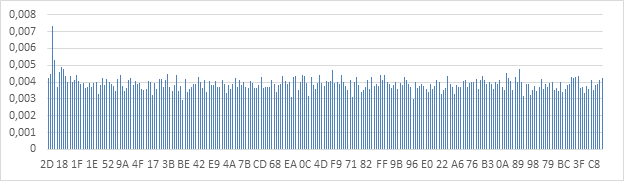
\includegraphics[natwidth=624bp,natheight=184bp,width=\linewidth]{histogram_meta}
\caption{Histogram showing frequency of each byte in Fitbit datadumps, Not corrected for the header and footer.}
\label{fig:histogram_meta}
\end{figure}

\begin{figure}
\noindent
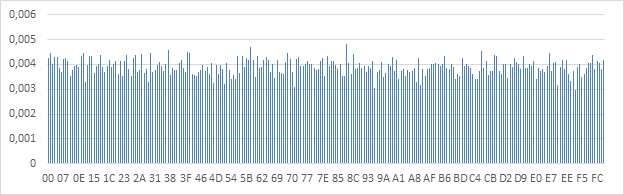
\includegraphics[natwidth=624bp,natheight=195bp,width=\linewidth]{histogram_nometa}
\caption{The same histogram as in fig.~\ref{fig:histogram_meta}, but corrected for header and footer information.}
\label{fig:histogram_nometa}
\end{figure}

But as figure~\ref{fig:histogram_meta} shows, there are some anomalies. The byte 00 appear to be overrepresented having a ratio of 0.7\%, but once we adjust for the 16-byte header and a 9-byte footer the result is much more even leaving us with a histogram of the data only (figure~\ref{fig:histogram_nometa}). There seems to be around one percent separating the most and least common byte, which suggests that Fitbit is using some kind of encryption and/or compression before sending the data from the device. According to a presentation made by French security researcher Axelle Aprville, Fitbit encrypts data on the tracker; the software running on the paired computer or smartphone doesn't decrypt the information but act as a relay towards Fitbit.com where it is assumed to be decrypted and further processed \citep{Aprville:2015a}. This is also supported by correspondence on the Galileo mailing list \citep{Allard:2014b}. Aprville mentions AES and XTEA as possible candidates for the encryption algorithm, but confirming this will be difficult with no access to the source code. The only method likely give us further insight would be to decompile the firmware on the device. Doing this can also safely be said to fall outside the scope of this article, so further research is needed for this approach.

\subsubsection{Integrity of the device data}
Assessing the integrity of the data at present can be regarded as difficult. There is currently no way to extract the data from our tracker, and no way of knowing what is left on the device after a dump has been extracted, or if the data is wiped from memory.


\subsection{Downloading data from the Fitbit API}
As mentioned earlier, Fitbit currently doesn't offer any way to download intraday data from the dashboard at Fitbit.com. They do offer an export service for daily averages, but for our purpose this is not useful.

The Fitbit API\footnote{https://dev.fitbit.com} in the form of a web service which can be used to access data. To use this API, you have to register an “app” with Fitbit. There are three types of apps; server, client and personal. All three have access to daily averages; the latter one also have access to the intraday data of the app owner. It is possible to obtain intraday data on the two former types of apps, but this requires individual approval from Fitbit as this also have the potential of allowing an app to access other user's data. (Fitbit 2014b)

To extract data from the Fitbit API we have to create a personal app using OAuth2 as the authorization framework, following the steps of the Implicit grant flow described in the Fitbit API documentation. The source code used to extract data is available under the BSD license on Github3, so we will skip the details of the implementation here. As implemented, the application created will retrieve steps taken, heart rate, distance walked, elevation calories burnt and number of floors climbed on a per-minute basis. This is not the complete set of data it is possible to extract, but as these data types have a common format it was easier for us to limit ourselves to them. It is also possible to extract various data related to sleep, food and water, as well as other types of data.

Data is received as JSON, separated by the type of data; the application merges the data obtained into a representation of a day divided into minutes as shown below.

\scriptsize
\begin{verbatim}
<minute time="18:53:00" steps="78" heartrate="98" distance="0" elevation="3" calories="8" floors="1" />
\end{verbatim}
\normalsize

While testing this, we were able to obtain data starting from the date our user account was created on Fitbit.com, up until the time of writing this. The start and end date can be specified when requesting data; so even with a large dataset it is possible to extract e.g. only the most recent 7 days.

The caveat of this method is of course that the data from the Fitbit tracker must be uploaded for this to work. Given our scenario this would require a murder victim to have a paired device nearby with an active network connection. Given that the device is designed to be used with a smartphone this isn't unlikely, but it is still a disadvantage for the investigators compared to extracting data directly from the device.

\subsubsection{Integrity of the API data}
One important issue is that the API supports methods for writing data as well as reading. Although writing data using the API wasn't tested, it is possible to see what apps a user has approved and their permissions. Figure~\ref{fig:apisettings} shows a screenshot from the Fitbit.com settings, showing the list of the authors approved apps. If we assume that investigators of a crime has access to the relevant Fitbit user accounts, a quick check on this page might give an indication if any registered apps have write access, and if so to what types of data.

\begin{figure}
\noindent
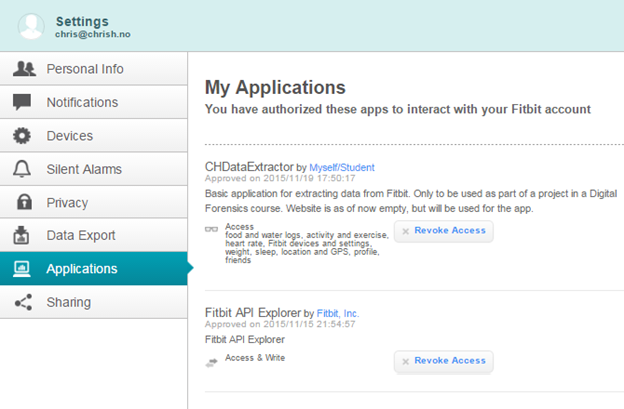
\includegraphics[natwidth=624bp,natheight=409bp,width=\linewidth]{apisettings}
\caption{List of approved apps from authors user account at Fitbit.com}
\label{fig:apisettings}
\end{figure}

Unfortunately there doesn't seem to be any way to see a historical record of approved or removed apps on the website or in the API. Therefore it is theoretically possible for a person to create their own app and use it to modify their data, removing and deleting the app from Fitbit once done. To verify such as case would likely require forensic examination of other computer equipment and/or cooperation from Fitbit itself.


\subsection{Extracting the data from a smartphone}

Similar to the device and dashboard, Fitbit doesn't offer any built-in functionality for extracting the data from the smartphone application. Although it might be possible to use adb backup to retrieve the data, this method is reliant upon the application supporting it. Another alternative, although more invasive is to gain root access on the phone which allows us to see (and copy) anything stored on it.

The smartphone used in this case is a Samsung Galaxy SIV, with an alternative version of Android installed called Cyanogenmod. The reason for having this instead of the stock version has no relation to the challenge at hand, it is simply a personal preference. Cyanogenmod does offer selective root access; apps can request root access, but the user have to approve it for each app. In this specific case it would appear that it is a non-invasive method as the smartphone was rooted before beginning to use the Fitbit tracker, and also as the only app authorized to have root access was the terminal application used to extract the app data. The extraction process was very basic:

\begin{enumerate}
\item Open the terminal, gain root access (\texttt{su -})
\item Navigate to the Fitbit app data directory, in this case \\ \texttt{/data/data/com.fitbit/FitbitMobile}
\item Package the entire directory using the builtin zip-command, saving the archive to the external SD-card
\item Copy the zip-file over to a computer
\end{enumerate}

As mentioned earlier in the article this is unlikely to apply to most other devices, as very few of them are rooted. (Google 2014) Our task is primarily to investigate what kind of data the smartphone holds, so the method used to extract the data is therefore regarded as less important. There have also been demonstrated vulnerabilities in Android such as CVE-2014-3153 giving elevated privileges; and the existence of such bugs cannot be ruled out as a non-invasive method to obtain data on a phone.

The data extracted from the app data directory consists of the following directories:

\vspace{1em}
\noindent
\texttt{app\_MixpanelAPI.Images}
\begin{itemize}
\item Empty directory.
\end{itemize}

\noindent
\texttt{app\_webview}
\begin{itemize}
\item Contains 2 databases: Cookies and Web Data.
\item No content related to tracker data or authentication towards the tracker in either.
\end{itemize}

\noindent
\texttt{cache}
\begin{itemize}
\item Contains two directories; \texttt{datacache} and \texttt{httpcache}.
\item \texttt{datacache} contains a mixture of images (jpeg, gif and png), and some json files. Based on the content of the images and the json data, this appears to be content shown in the Fitbit app. Obvious clues here are the json files containing what appear to be setup wizards with various steps to help the user connect and pair the trackers.
\item \texttt{httpcache} contains a cached http request dating from November 6; this date is not special in any way. Data capture using the tracker started on November 5.
\item \texttt{httpcache} also contains the file \texttt{journal}, which seems to be related to something called \texttt{DiskLruCache}. Based on the available Android documentation this might be related to the data in datacache.
\item Also contains a binary file; \texttt{com.android.opengl.shaders\_cache} which seems to be related to the graphics.
\end{itemize}

\noindent
In addition to these, we also found directories called \texttt{databases}, \texttt{files} and \texttt{shared\_prefs}. Based on the content these deserve a more detailed description.

\subsubsection{\texttt{databases}}
The folder \texttt{databases} contains 13 SQLite databases, plus one backup journal file for each. Most of the databases appear to be empty, although some information was found.

\begin{description}
\item [Alarm] The Fitbit Charge HR has the ability to set alarms, but must be programmed using the smartwatch. I have one alarm set to 06:45 in the morning; in a database \texttt{fitbit\_db} under the table \texttt{alarm}, I found a row with the timestamp “1448430300000”. This would appear to be too long to be a regular unix timestamp, but by removing two zeroes to the right I get a timestamp for 25.11.2015 05:45 UTC. The data was extracted from the phone on November 24; UTC is one hour behind my timezone so the corrected time is 06:45. This would therefore appear to be the next alarm set on the device.
\item [Device] The same database holding the Alarm also has a device table listing columns such as a timestamp for “last sync time”, but it is unknown if this refers to the tracker or the smartphone app. It also holds columns named \texttt{encoded\_id}, \texttt{wire\_id}, version information related to the current firmware on the tracker as well as version information for a new version of the firmware.

I also see the MAC address of the tracker; this is also displayed when using Galileo to perform extracts, so it would appear to be possible to link a smartphone with a specific tracker.
\item [Profile] The profile table contains information related to the user logged in to the smartphone app. This contains various bits of personal information, such as weight and height, along with some fields that are set automatically such as stride length while running and walking. These values are presumably calculated based on user height and other values. Interestingly this table has a column containing an \texttt{encoded\_id}. The value in this field cannot be found in any of the other files or databases extracted, so the purpose of this is unknown. There is also columns for an OAuth token and secret, although these hold no data at the moment.
\item [Time\_Series\_Object] While this table doesn't hold any information that seems to be important, it is worth noting that it lists a number of timestamps, some of which are prior to registering with Fitbit. Most days have one or more records with a timestamp pointing to 11AM on a given day; but every few days there are a lot of records with timestamps pointing to nighttime. There appears to be a pattern of one or two timestamps with a minute or so interval, and then either $\sim$20 minutes or $\sim$70-90 minutes until a new set of timestamps. This does not appear to be relevant, but it could be valuable if combined with additional data.
\item [Sleep\_Log\_Entry] This table is contained in the logging\_db file, and appears to list a record of sleep as captured by the tracker. Based on the column headings this gives me the following data for November 13:
\begin{itemize}
\item I went to sleep at 01:36
\item I slept for 5 hours 16 minutes, but I was in bed for 5 hours 24 minutes
\item I didn't wake up properly during the night but was about to do so twice and was restless twice
\item According to Fitbit this was not my main sleep, but it had an efficiency of 98\%.
\end{itemize}
The overall impression of these databases is that there is room for a lot of data not present in our extract. If this is due to the method used to extract the data, or simply because the databases aren't used at present is unknown. But this is something that should be investigated further.
\end{description}


\subsubsection{\texttt{files}}

This directory contains four files:

\begin{itemize}
\item \texttt{authinfo\_credentials.json}
\item \texttt{trackerAuthCredentials.json}
\item \texttt{gaClientId}
\item \texttt{gaClientIdData}
\end{itemize}

\noindent
The two json files doesn't contain valid json, but rather something looking like encryption keys with lengths of 128 and 152 characters:

\scriptsize
\begin{itemize}
\item \texttt{Ey+ydbyoIgAjKTNjZ18NnMQe263m ... (snip) ... aWrG7XfmMI/kDIKOEEpi/kmi/+MdyxhzTDpRPsSq}
\item \texttt{7MfLXxn3a5RHwHJlSa0kBqMRoZx ... (snip) ... n4pB+THsOjGE4xlDEepRc+AZy6cvfQB7afAC5dg==}
\end{itemize}
\normalsize

\noindent
\texttt{gaClientId} contains something looking like a GUID. This does not match any GUIDs found in any of the databases, so the purpose of this is unknown. \texttt{gaClientIdData} contains what appears to be a 16-byte hexadecimal string.

\subsubsection{\texttt{shared\_prefs}}
This directory contains 35 XML-files, with quite a lot of them being simple configuration files with little content. Some holds information related to other services, such as Google Cloud Messaging (GCM), where we can find the attribute regId containing a 140 character key. This might be some sort of a user or client ID used to identify my specific user account, the Fitbit tracker, smartphone app or Fitbit itself towards GCM. It doesn’t appear to be relevant for us, but it could be important for an investigation depending on the scope.

There is also a file called \texttt{com.facebook.internal.preferences.} \\ \texttt{APP\_SETTINGS.xml}. It is important to mention that the author originally connected Fitbit and Facebook too see how the social and competitive aspect of the Fitbit Dashboard worked, but this link was broken before making this extract. At the moment this doesn’t hold any information related to my Facebook profile, but this could be worth investigating further.

The file \texttt{TrackerSync.xml} holds a number of timestamps, which looks like a list of various times certain events happened, such as last tracker boot, last sync and similar. What is surprising here is that there is four references to something called “Galileostate” and background synchronization. This might be a random occurrence, but the fact that the tool used to extract dumps from the device is called Galileo is a bit of a coincidence. There are no links between the Fitbit app on the smartphone and Galileo running inside a virtual Linux computer other than the Fitbit tracker. This might suggest that Galileo leaves information on the tracker or that the tracker logs these requests.

Then there is a file \texttt{LiveDateSavedState.xml} containing the last set of live data. Based on the values these appear to be a cumulative dataset; there is no timestamp on the data however so time framing these data would be difficult.

\subsubsection{Integrity of the extracted data}
The data was extracted by adding a number of files to a zip-file. As the smartphone was rooted before we began this project, this shouldn’t affect the integrity.


\subsection{Conclusion}

Based on what we have observed through our own testing extracting useable data from the device isn’t possible at the moment. The data retrieved from the tracker is likely to be encrypted with an unknown algorithm and key; this also correlates with what others have experienced. If retrieving data directly from the device is critical to an investigation, the only likely approach is to request help from Fitbit.

Extracting data from the API is possible and have been demonstrated during this project. To access data owned by any other profile but your own requires Fitbit approval as well as user approval. As seen from a forensic point-of-view this would require access to the Fitbit user account in question in order to be a useable approach. If this is the case however; it should be possible to sync a tracker holding important information with Fitbit, and then access the same data through the API.

Although the data extracted from the smartphone didn’t give us any minute-by-minute data, it did give us some interesting information related to keys and IDs. More research is needed to determine if any of the key-like values found can be used in any way to decrypt data from the Fitbit tracker or if they can be used against the API. However, in \cite{Snyder:2015} an essential bit of information was the fact that the alleged rape victim didn’t sleep during the night. In this project we were able to extract similar information from the smartphone. Despite not being able to extract data directly from the tracker, a forensic analysis of paired devices can still give valuable information without having to know or access the users own account on Fitbit.com. Our analysis was from the files stored on disk; a more in depth analysis may reveal more information stored in volatile memory on the device.

Although more research is needed into the data being sent from the tracker and the data stored on a paired smartphone, it would appear that even a superficial analysis such as ours can be beneficial to investigators. We managed to find a connection between the physical tracker and a smartphone; and from the smartphone to the e-mail address used when registering with Fitbit.com.

Even though we couldn’t extract as much information from the device or smartphone as we had hoped, there still appears to be viable approaches for getting this information out of the tracker if it is allowed to upload data to Fitbit.com.


\section{Discussion}

\textit{We'll probably need to cooperate on this one. We can all write a small discussion on the devices we've looked at, and one of us can try to mold that into a single conclusion with some words of comparison between the devices. In any case, we need to write the above section first.}

\bibliographystyle{agsm}
\bibliography{forensics.bib}

\end{document}
